\chapter{TADAS阻尼器}
在本章中对工程实际应用中常见的三角形板(TADAS)阻尼器进行介绍,随后通过数值建模对其进行数值分析,详细对比使用罚函数法、Nitsche法和HR法的位移云图,证明所提方法在解决工程实践应用问题具有一定的优势。
\section{TADAS阻尼器}
在建筑和工程结构中,振动是一个常见的问题,其可能会导致结构的疲劳破坏等问题,传统方法中通过采用增加结构的刚度或使用液体阻尼器、摩擦阻尼器减小结构的振动响应,然而在传统方法中或多或少的存在有效性不高,经济适用性低等问题。
为了克服传统方法的限制,三角板减振刚度阻尼器被引入(TADAS),TADAS阻尼器是一种基于能量耗散原理的被动控制装置,通过在结构中引入附加的阻尼力来吸收和耗散结构的振动能量,能够有效地减小结构地的振动幅值和振动周期,从而显著改善结构的振动响应,
并且TADAS阻尼器的设计相对简单,通常由一块或多块金属材料制成,安装简易、价格低廉,是一种在结构工程中广泛应用于减震和控制结构的被动控制装置。\par
图(\ref{TADAS1})为一个带有TADAS阻尼器的实验装置\textsuperscript{\cite{mohammadi2017,kim2016}},为常在道路、住房和城市中心建造的一层框架大比例模型,
该框架高3米,跨度4米,框架柱采用标准的双IPE180型钢材,梁的工字截面由三块4000*200*12mm的钢板连续焊接而成。支撑体系统一采用双100*100*20mm角度,柱基座使用销连接。
如图(\ref{TADAS2})所示,TADAS阻尼器中的三角形板的上端设为简支固定,下端施加$P=100000$的力。三角形钢板的材料系数为杨氏模量$E=2\times 10^{11}$、泊松比$\nu=0.3$。
\begin{figure}[H]
    \centering
    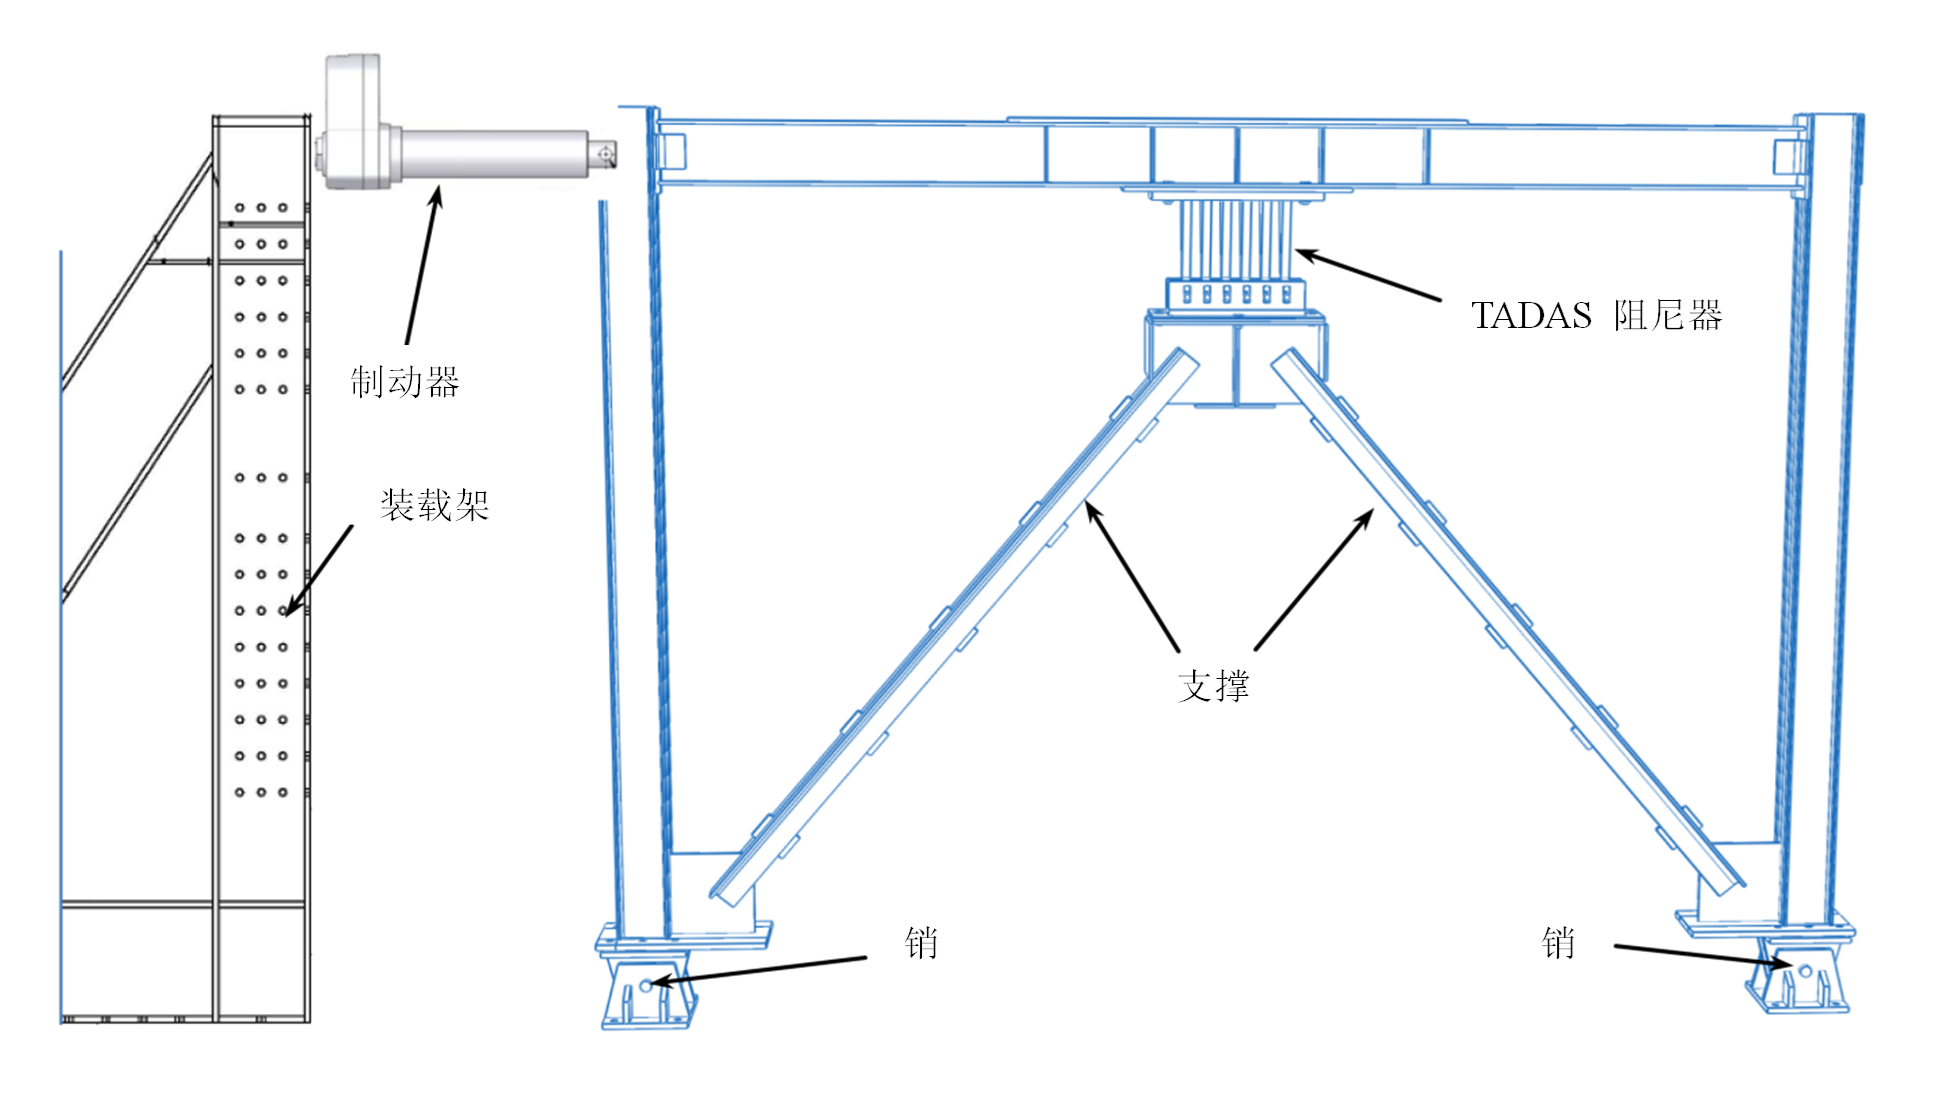
\includegraphics[scale=0.4]{figure/TADAS/1.png}
    \caption{实验装置示意图}\label{TADAS1}
\end{figure}
\begin{figure}[H]
    \centering
    \begin{subcaptiongroup}
            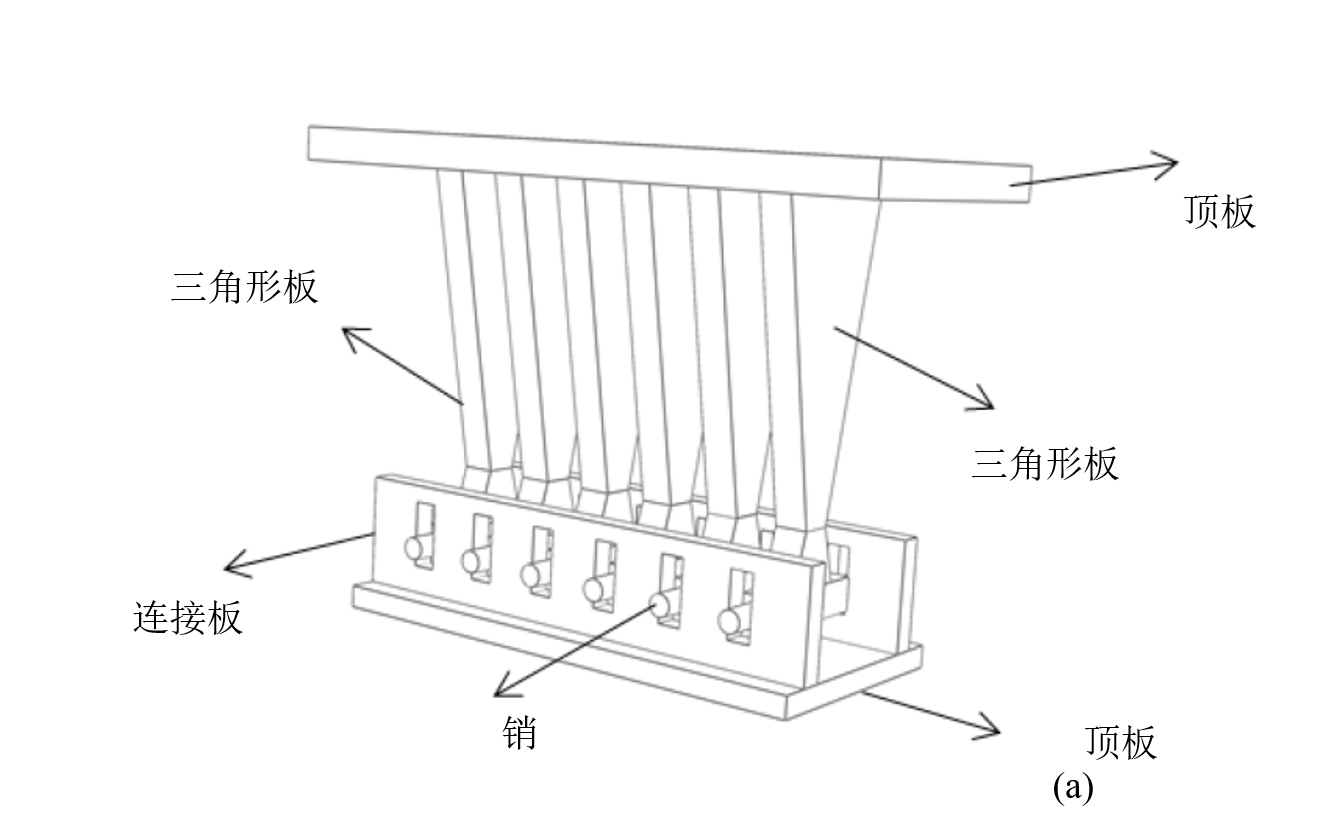
\includegraphics[width=0.69\textwidth]{figure/TADAS/2.png}
            \phantomcaption\label{TADAS2}
            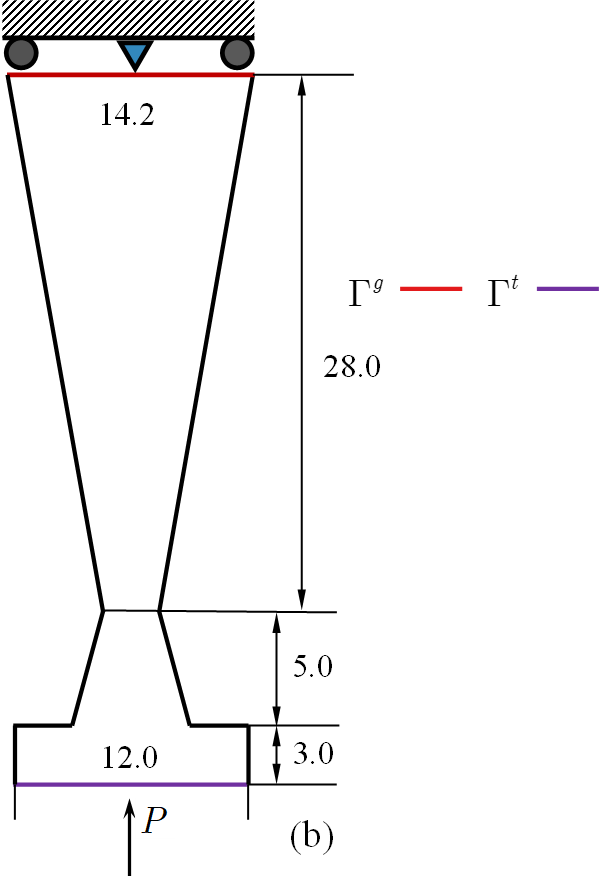
\includegraphics[width=0.29\textwidth]{figure/TADAS/3.png}
            \phantomcaption\label{TADAS3}
            \end{subcaptiongroup}
        \caption{TADAS阻尼器示意图:\subref{TADAS2} 钢板焊接TADAS装置详图;\subref{TADAS3} 三角形钢板横截面图}
    \label{TADAS2}
\end{figure}
图(\ref{TADAS4})为TADAS阻尼器三角形板的位移应力云图,从图中可以看出所提方法“HR”法的计算结果与常见解决薄板实际应用问题的方法“Nitsche”法和罚函数法具有几乎相同的位移结果,说明我们所提出的新方法能够解决工程实践应用薄板问题。
\begin{figure}[H]
    \centering
    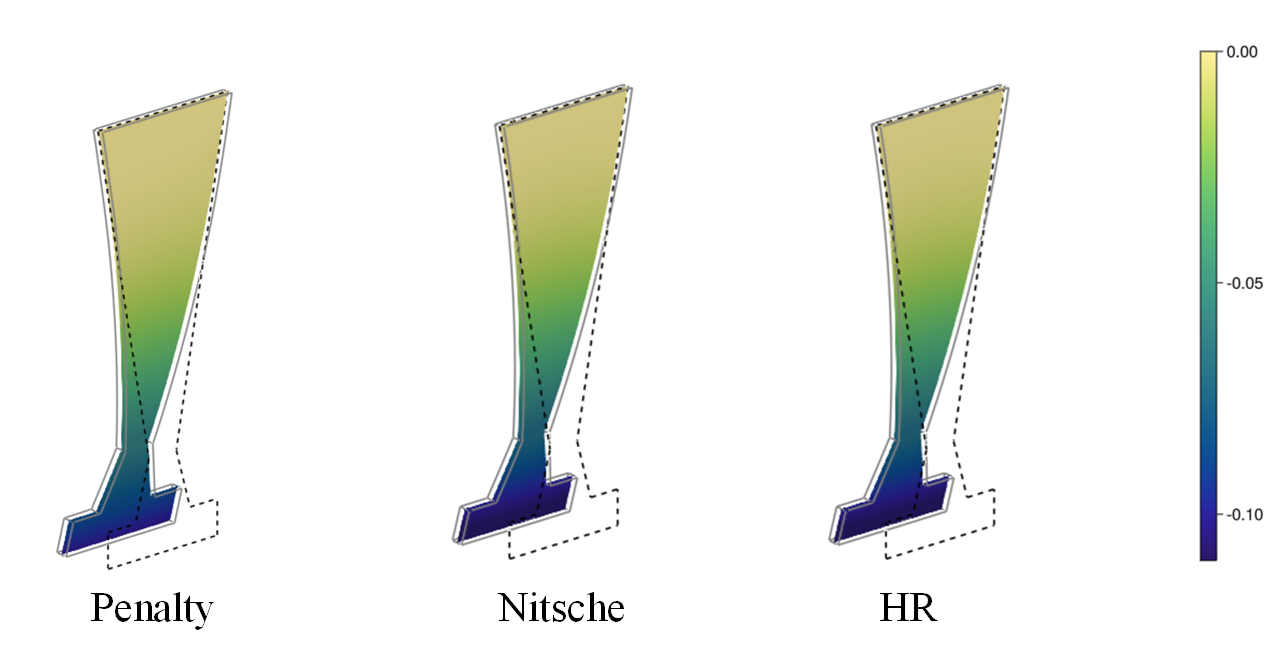
\includegraphics[scale=0.5]{figure/TADAS/4.png}
    \caption{TADAS阻尼器位移云图}\label{TADAS4}
\end{figure}
\section{小结}
本章首先对TADAS阻尼器的优点进行详细介绍,随后对一个一层框架大比例模型中带有TADAS阻尼器进行数值分析,通过采用不同的本质边界条件施加方法-罚函数法、Nitsche法和本论文所提方法HR法得到的位移云图进行分析,
得出基于Hellinger-Reissner变分原理的变分一致性伽辽金无网格法能够有效处理解决工程实际中的薄板模型,为薄板问题的工程数值分析提供了一种新思路。


